\chapter{Proxy}

\section{Definici'on}

Los servidores proxy son Intermediarios. Se encuentran entre el cliente y el servidor, act'ua enviando los mensajes del cliente al servidor y viceversa. En una comunicaci�n normal, le cliente se comunica directamente con el servidor, en el caso de que en la red haya un proxy presente, el cliente se comunica con el proxy y este es el que se comunica con el servidor.

\begin{figure}[ht!]
  	\centering
	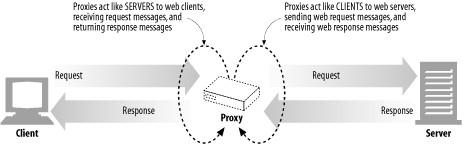
\includegraphics[width=\textwidth]{img/proxy_1}
	\caption{\small Esquema del funcionamiento de un Proxy, extra'ido de \cite{httpGuide}}
	\label{proxy_1}
\end{figure}

El proxy es un web server y tambi'en es cliente. Para recibir los pedidos de los clientes, tiene que actuar como un servidor y manejar correctamente las peticiones, conexiones y respuestas. A su vez, para poder conectarse a los destinos finales y recuperar los recursos que le son pedidos por el usuario del proxy, tiene que actuar como un cliente, enviando peticiones y recibiendo las respuestas. Se puede ver el funcionamiento b'asico de un Proxy en la Figura \ref{proxy_1}.

El esquema de la Figura \ref{proxy_1} muestra una conexi'on utilizando HTTP, las peticiones viajan directamente al Proxy y de ah'i al servidor final. En el caso de HTTPS se hace de manera diferente. Primero el Cliente env'ia una petici'on con el M'etodo CONNECT que incluye la direcci'on y el puerto del destino final. El proxy autentica la conexi'on, completa la negociaci'on con el destino y responde al cliente con un mensaje que contiene el c'odigo 200 que indica que la conexi'on fu'e establecida. Luego, el proxy se convierte en un t'unel que solo reenv'ia los paquetes del cliente hacia el servidor y viceversa (todo el tr'afico se encuentra encriptado). Esto puede ilustrarse en la Figura \ref{proxy_2}. Los browsers actuales no soportan Proxies HTTP Seguros, es decir, que se establezca una sesi'on SSL del Cliente al Proxy y otra del Proxy al Servidor Final como puede verse en la Figura \ref{trustedProxy}. Este 'ultimo punto est'a en discusi'on, se propuso un borrador \citep{draftTrustedProxy} al respecto.

\begin{figure}[h]
  	\centering
	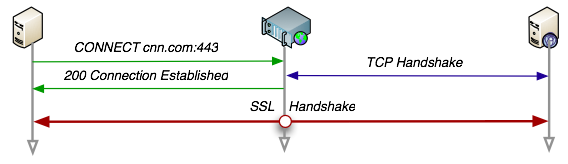
\includegraphics[width=\textwidth]{img/proxy_2}
	\caption{\small T'unel HTTPS sobre un Proxy, extra'ido de \cite{secureProxies}}
	\label{proxy_2}
\end{figure}

\begin{figure}[h]
  	\centering
	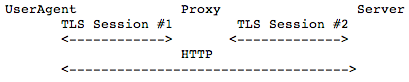
\includegraphics[width=\textwidth]{img/trustedProxy}
	\caption{\small T'unel HTTPS sobre un Proxy, extra'ido de \cite{draftTrustedProxy}}
	\label{trustedProxy}
\end{figure}

\section{Usos de un Proxy}

Hay diversas utilizaciones de los servidores proxy, entre ellas se destacan:

\begin{enumerate}
\item Filtro

El Proxy al recibir las peticiones de los clientes, puede permitir o denegar esas peticiones seg'un ciertas pol'iticas definidas. Por ejemplo, en una Instituci'on Educativa se podr'ia bloquear el acceso a ciertas redes sociales o sitios para adultos.

\item Cortafuegos\footnote{Firewall}

Al ser un intermediario, y muchas veces como puerta de acceso hacia internet, se pueden utilizar para aumentar el nivel de seguridad restringiendo ciertos protocolos o filtrando cierto contenido inseguro por ejemplo.

\item Web Cach'e

Puede mantener copias locales de los recursos peticionados por los clientes, al servir varios clientes esto incrementa la velocidad de respuesta. Esto se ver'a detalladamente en el Cap'itulo \ref{cache}.

\item Proxy Reverso / Surrogate Server

Puede actuar delante de un Servidor Web, atendiendo peticiones de los clientes como si fuera 'el Servidor mismo. Esto permite por ejemplo, generar una Red de Distribuci'on de Contenidos\footnote{CDN}. Recibe una petici'on de un cliente, y, en vez de devolver el contenido directamente, inicia una comunicaci'on con otros servidores para localizar el recurso pedido de manera m'as eficiente. Tambi'en protege a los Servidores Web, a'nadiendo una capa adicional de defensa. Puede distribuir la carga entre varios Servidores Web.

\item Content-Router

Pueden redirigir las peticiones a Servidores basados en las condiciones del Tr'afico de Internet y el tipo de contenido. REVISAR

\item Transcoder

Puede modificar el contenido de los recursos antes de hacer el env'io a los clientes. Por ejemplo, transformar im'agenes BMP a JPEG para reducir el tama'no, comprimir archivos de texto, e incluso hacer una traducci'on del contenido a otro lenguaje.

\item Anonimizador

Permite navegar de manera privada y an'onima removiendo ciertos datos de los mensajes HTTP (Direcci'on IP, From Header, cookies, etc).

\end{enumerate}

\subsection{Configuraci'on}

Existen varias maneras de configurar un browser para navegar a trav'ez de un Proxy.

\section{SPDYProxy}

FALTA: EXPLICAR FUNCIONAMIENTO DEL SPDYPROXY

